\subsection{co limits}

\begin{frame}
Let $\mathcal{C}$ be a category. A {\it diagram} in $\mathcal{C}$ is a functor $M : \mathcal{I} \to \mathcal{C}$. $\mathcal{I}$ is the {\it index category} and $M$ is an $\mathcal{I}$-diagram. $M_i$ denotes the image of the object $i$ of $\mathcal{I}$ in $\cC$. For $\phi : i \to i' \in \Mor(I)$, $M(\phi) : M_i \to M_{i'}$.
\end{frame}

\begin{frame}
\iftoggle{thmsty}{
\begin{definition}
\label{definition-limit}
}{}
A {\it limit} of the $\mathcal{I}$-diagram $M$ in the category
$\mathcal{C}$ is given by an object $\lim_I M$ in $\mathcal{C}$
together with morphisms $p_i : \lim_I M \to M_i$ such that
\begin{enumerate}
\item for $\phi : i \to i'$ a morphism
in $\mathcal{I}$ we have $p_{i'} =  M(\phi) \circ p_i$, and
\item for any object $W$ in $\mathcal{C}$ and any family of
morphisms $q_i : W \to M_i$ such that for all $\phi : i \to i'$
in $\mathcal{I}$ we have $q_{i'} = M(\phi) \circ q_i$ there
exists a unique morphism $q : W \to \lim_I M$ such that
$q_i = p_i \circ q$ for every object $i$ of $\mathcal{I}$.
\end{enumerate}
\iftoggle{thmsty}{
\end{definition}
}
\end{frame}

\begin{frame}
\noindent These conditions are expressed in the commutativity of the diagram
\begin{displaymath}
\xymatrix{
&\ar[ldd]_{q_i} W \ar@{-->}[d]^{q} \ar[rdd]^{q_{i'}} & \\
& \ar[ld]^{p_i} \lim\limits_{\longleftarrow \mathcal{I}} M \ar[rd]_{p_{i'}} &\\
M_i  \ar[rr]_{M(\phi)} & & M_{i'} \\
i \ar[rr]^{\phi} & & i'  
}
\end{displaymath}
\end{frame}

\begin{frame}
\noindent
Limits $(\lim_I M, (p_i)_{i\in \Ob(\mathcal{I})})$ are unique up to unique isomorphism, if they exist at all, according to the uniqueness requirement in the definition. Products of pairs and equalizers are examples of limits. The limit over the empty diagram is a final object of $\cC$. In the category of sets all limits exist. The dual notion is that of colimits.
\end{frame}

\begin{frame}
\iftoggle{thmsty}{
\begin{definition}
\label{definition-colimit}
}{}
A {\it colimit} of the $\mathcal{I}$-diagram $M$ in the category
$\mathcal{C}$ is given by an object $\colim_I M$ in $\mathcal{C}$
together with morphisms $s_i : M_i \to \colim_I M$ such that
\begin{enumerate}
\item for $\phi : i \to i'$ a morphism
in $\mathcal{I}$ we have $s_i = s_{i'} \circ M(\phi)$, and
\item for any object $W$ in $\mathcal{C}$ and any family of
morphisms $t_i : M_i \to W$ such that for all $\phi : i \to i'$
in $\mathcal{I}$ we have $t_i = t_{i'} \circ M(\phi)$ there
exists a unique morphism $t : \colim_I M \to W$ such that
$t_i = t \circ s_i$ for every object $i$ of $\mathcal{I}$.
\end{enumerate}
\iftoggle{thmsty}{
\end{definition}
}
\end{frame}

\begin{frame}
\noindent These conditions are expressed in the commutativity of the diagram

\begin{displaymath}
\xymatrix{
i \ar[rr]^{\phi} & & i' \\
M_i \ar[rd]^{s_i} \ar[rdd]_{t_i} \ar[rr]^{M(\phi)} & & M_{i'} \ar[ldd]^{t_{i'}} \ar[ld]_{s_{i'}}\\
& \lim\limits_{\longrightarrow \mathcal{I}} M \ar@{-->}[d]^{t}& \\
& W &
}
\end{displaymath}
\end{frame}

\begin{frame}
\noindent
Colimits $(\colim_I M, (s_i)_{i\in \Ob(\mathcal{I})})$ are unique up to unique isomorphism by the uniqueness requirement in the definition. Coproducts of pairs and coequalizers are examples of colimits. The colimit over an empty diagram is an initial object of $\mathcal{C}$. All colimits exist in the category of sets.
\end{frame}

\begin{frame}
Combining the diagrams for limit and colimit (in general the objects W refer to different objects in each diagram) demonstrates the reason that limits are often referred to as {\it cones over} a diagram and colimits are referred to as {\it cocones under} a diagram
\end{frame}

\begin{frame}
\begin{displaymath}
\xymatrix@=17pt{
&\ar[ldd]_{q_i} W \ar@{-->}[d]^{q} \ar[rdd]^{q_{i'}} & \\
& \ar[ld]^{p_i} \lim\limits_{\longleftarrow \mathcal{I}} M \ar[rd]_{p_{i'}} &\\
M_i  \ar[rr]_{M(\phi)} & & M_{i'} \\
i \ar[rr]^{\phi} & & i' \\
M_i \ar[rd]^{s_i} \ar[rdd]_{t_i} \ar[rr]^{M(\phi)} & & M_{i'} \ar[ldd]^{t_{i'}} \ar[ld]_{s_{i'}}\\
& \lim\limits_{\longrightarrow \mathcal{I}} M \ar@{-->}[d]^{t}& \\
& W &
}
\end{displaymath}
\end{frame}

\subsection{functors and equivalence}

\begin{frame}
We can define a category having functors as objects and natural transformations as morphisms, which is called a functor category, by recognizing that every functor $F$ comes with the {\it identity} transformation $\text{id}_F : F \to F$. In addition, given a morphism of
functors $t : F \to G$ and a morphism of functors $s : E \to F$
then the {\it composition} $t \circ s$ is defined by the rule
$$
(t \circ s)_x = t_x \circ s_x : E(x) \to G(x)
$$
for $x \in \Ob(\mathcal{A})$.
This is a morphism of functors
from $E$ to $G$.
Thus, given categories
$\mathcal{A}$ and $\mathcal{B}$ we obtain the category of functors between $\mathcal{A}$ and
$\mathcal{B}$.
\end{frame}

\begin{frame}
\iftoggle{thmsty}{
\begin{definition}
\label{definition-equivalence-categories}
}{}
An {\it equivalence of categories}
$F : \mathcal{A} \to \mathcal{B}$ is a functor such that there
exists a functor $G : \mathcal{B} \to \mathcal{A}$ such that
the compositions $F \circ G$ and $G \circ F$ are isomorphic to the
identity functors $\text{id}_\mathcal{B}$,
respectively $\text{id}_\mathcal{A}$.
In this case we say that $G$ is a {\it quasi-inverse} to $F$.
\iftoggle{thmsty}{
\end{definition}
}
\end{frame}

\subsection{adjunctions}

\begin{frame}
\iftoggle{thmsty}{
\begin{definition}
\label{definition-adjoint}
}{}
Let $\mathcal{C}$, $\mathcal{D}$ be categories.
Let $u : \mathcal{C} \to \mathcal{D}$ and
$v : \mathcal{D} \to \mathcal{C}$ be functors.
We say that $u$ is a {\it left adjoint} of $v$ or that
$v$ is a {\it right adjoint} to $u$, written $u \dashv v$, if there are bijections
$$
\phi_{X,Y}:\Mor_\mathcal{D}(u(X), Y)
\simeq
\Mor_\mathcal{C}(X, v(Y))
$$
functorial in $X \in \Ob(\mathcal{C})$, and
$Y \in \Ob(\mathcal{D})$.
\iftoggle{thmsty}{
\end{definition}
}
\end{frame}

\begin{frame}
Morphisms that are associated with each other according to the bijections of an adjunction are called {\it adjoint transposes} of one another. If $g:u(X) \rightarrow Y$, $g \in \Mor(\mcD)$ then $g^*: X \rightarrow v(Y)$, $g^* \in \Mor(\cC)$ is given by $\phi_{X,Y}(g) = g^*$. Similarly for $f: X \rightarrow v(Y)$, $f \in \Mor(\cC)$ with $f^*:u(X) \rightarrow Y$, $f^* \in \Mor(\mcD)$ is given by $\phi_{X,Y}^{-1}(f) = f^*$. We see then that $g^* = f$ and $f^* = g$.
\end{frame}

\begin{frame}
\iftoggle{thmsty}{
\begin{definition}
\label{definition-opposite}
}{}
Given a category $\mathcal{C}$ the {\it opposite category}
$\mathcal{C}^{opp}$ is the category with the same objects
as $\mathcal{C}$ but all morphisms reversed.
\iftoggle{thmsty}{
\end{definition}
}
\end{frame}

\begin{frame}
\iftoggle{thmsty}{
\begin{definition}
\label{definition-contravariant}
}{}
Let $\mathcal{C}$, $\mathcal{S}$ be categories.
A {\it contravariant} functor $F$
from $\mathcal{C}$ to $\mathcal{S}$
is a functor $\mathcal{C}^{opp}\to \mathcal{S}$.
\iftoggle{thmsty}{
\end{definition}
}
\end{frame}

\begin{frame}
\iftoggle{thmsty}{
\begin{definition}
\label{definition-presheaf}
}{}
Let $\mathcal{C}$ be a category.
\begin{enumerate}
\item A {\it presheaf of sets on $\mathcal{C}$}
or simply a {\it presheaf} is a contravariant functor
$F$ from $\mathcal{C}$ to $\textit{Sets}$. When $F$ is a covariant functor $F : \mathcal{C}^{opp} \rightarrow \textit{Sets}$.
\item The category of presheaves is denoted $\textit{PSh}(\mathcal{C})$.
\end{enumerate}
\iftoggle{thmsty}{
\end{definition}
}
\end{frame}

\subsection{bifunctors and homs}

\begin{frame}
\iftoggle{thmsty}{
\begin{definition}
\label{definition-bifunctor}
}{}
Given categories $\mathcal{C}_1$, $\mathcal{C}_2$, and $\mathcal{D}$. A {\it bifunctor} or binary functor or 2-ary functor or functor of two variables, $F$, is a functor whose domain is the product of two categories $F: \mathcal{C}_1 \times \mathcal{C}_2 \rightarrow \mathcal{D}$.
\iftoggle{thmsty}{
\end{definition}
}
\end{frame}

\begin{frame}
\iftoggle{thmsty}{
\begin{definition}
\label{definition-hom-functor}
}{}
The {\it hom-functor} is a bifunctor defined on the product of a category $\mathcal{C}$ with its self-dual category $\mathcal{C}^{opp}$, which takes values in the category $\textit{Sets}$. Thus for a category $C$ its hom-functor is 
$$
hom(-,-): \mathcal{C}^{opp} \times \mathcal{C} \rightarrow \textit{Sets},
$$
which can be curried in two ways
\begin{eqnarray*}
h^{(-)} &:& \mathcal{C}^{opp} \rightarrow \textit{Sets}^{\mathcal{C}},\\
h_{(-)} &:& \mathcal{C} \rightarrow \textit{Sets}^{\mathcal{C}^{opp}}.
\end{eqnarray*}
\end{frame}

\begin{frame}
The hom-functor maps
\begin{enumerate}
\item objects $(c,c') \in \mathcal{C}^{opp} \times \mathcal{C}$ to the hom-set $\Mor_{\mathcal{C}} (c,c')$, which is the set of morphisms in $\mathcal{C}$ with domain $c$ and codomain $c'$.
\item morphisms 
$$
(f,g):(c,c') \rightarrow (d,d') \in \Mor(\mathcal{C}^{opp} \times \mathcal{C}),
$$
where $f:d \rightarrow c \in \Mor(\mathcal{C})$ and $g:c' \rightarrow d' \in \Mor(\mathcal{C})$, to the set function
\begin{eqnarray*}
\Mor_{\mathcal{C}}(c,c') &\rightarrow& \Mor_{\mathcal{C}}(d,d')\\
(c \rightarrow c') &\mapsto& (d \rightarrow c \rightarrow c' \rightarrow d')
\end{eqnarray*}
\end{enumerate}
\iftoggle{thmsty}{
\end{definition}
}
\end{frame}

\begin{frame}
\iftoggle{thmsty}{
\begin{definition}
\label{definition-representable-functor}
}{}
For a hom-functor $hom(-,-): \mathcal{C}^{opp} \times \mathcal{C} \rightarrow \textit{Sets}$ for $c \in \Ob(\mathcal{C})$ a covariant and contravariant functor can be derived by specializing the hom-functor to morphisms out of or into the object $c$ as
\begin{eqnarray*}
h^c \equiv hom(c,-) &:& \mathcal{C} \rightarrow \textit{Sets},\\
h_c \equiv hom(-,c) &:& \mathcal{C}^{opp} \rightarrow \textit{Sets}.
\end{eqnarray*}
Functors that are isomorphic to $h^c$ or $h_c$ are referred to as {\it corepresentable or representable functors} respectively and $c$ is their {\it representing object}. Note that $h_c \in \Ob(\textit{PSh}(\mathcal{C}))$ and the Yoneda embedding states that $h_c$ extends to a functor $PSh : \mathcal{C} \rightarrow \textit{Sets}^{\mathcal{C}^{opp}}$ that is guaranteed to be full and faithful thereby having $\mathcal{C}$ as a full subcategory of the functor category $\textit{Sets}^{\mathcal{C}^{opp}}$ by the Yoneda lemma.
\iftoggle{thmsty}{
\end{definition}
}
\end{frame}

\begin{frame}
\begin{figure}
\noindent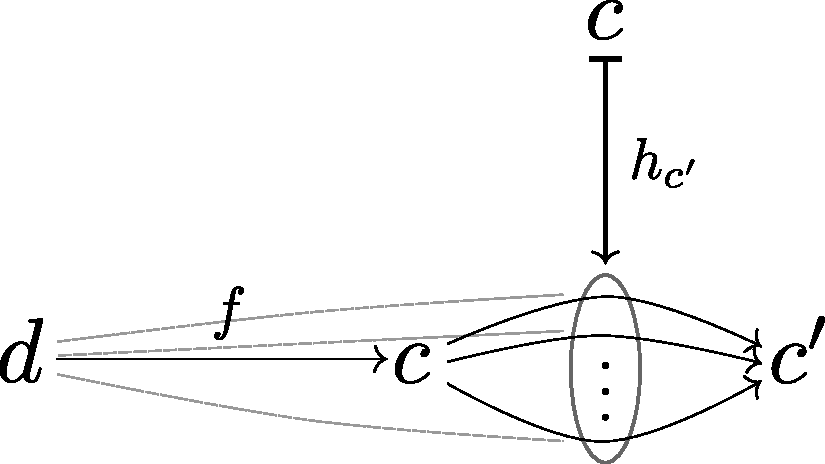
\includegraphics[width=0.7\framewidth]{fig/hom.pdf}
\caption{The presheaf represented by $c' \in \Ob(\cC)$ is $h_{c'} : \cC^{opp} \rightarrow \textit{Sets}$. It sends objects to the set of morphisms in which they are the domain object with codomain $c'$ and morphisms $f:d \rightarrow c \in \Mor{\cC}$ to set functions $h_{c'} \circ f: \Mor_{\cC}(c,c') \rightarrow \Mor_{\cC}(d,c')$ via pre-composition.}
\label{fig:hom}
\end{figure}
\end{frame}

%\begin{frame}
%The concrete action of $h_{c'}$ on objects and morphisms in $\cC$ is summarized in figure \ref{fig:hom}. The preceding definitions are standard category theoretic constructions. Ellerman has proposed an interpretation of adjoint functors, that demonstrates their relevance to the concept of information encoding and decoding (or sending and receiving) in the context of biological systems \cite{Ellerman2005}.
%\end{frame}

\begin{frame}
\iftoggle{thmsty}{
\begin{definition}
\label{definition-birepresentable}
}{}
A bifunctor $bif (-,-): \cC^{opp} \times \mcD \rightarrow \textit{Sets}$ is said to be {\it birepresentable} if there exists a pair of functors $F:\cC^{opp} \rightleftarrows \mcD:G$ where $c \in \Ob(\cC^{opp})$ and $d \in \Ob(\mcD)$ gives
\begin{eqnarray*}
b^{c} \equiv bif(c,-) &:& \mathcal{D} \rightarrow \textit{Sets},\\
b_{d} \equiv bif(-,d) &:& \mathcal{C}^{opp} \rightarrow \textit{Sets}.
\end{eqnarray*}
natural in $c$ and $d$ such that $F \dashv G$. The functors $b^{c}$ and $b_{d}$ are defined on
\begin{enumerate}
\item objects for all $c_i \in \Ob(\cC^{opp})$ and for all $d_i \in \Ob(\mcD)$
\begin{eqnarray*}
b^{c} (d_i) &=& \Mor_{\mcD}(Fc,d_i),\\
b_{d} (c_i) &=& \Mor_{\cC^{opp}}(c_i,Gd).
\end{eqnarray*}
\item morphisms for all $f_{ij}:c_j \rightarrow c_i \in \Mor(\cC^{opp})$ and for all $g_{ij}:d_i \rightarrow d_j \in \Mor(\mcD)$ as
\begin{eqnarray*}
b^{c} (g_{ij}) &:& \Mor_{\mcD}(Fc,d_i) \rightarrow \Mor_{\mcD}(Fc,d_j),\\
b_{d} (f_{ij}) &:& \Mor_{\cC^{opp}}(c_i,Gd) \rightarrow \Mor_{\cC^{opp}}(c_j,Gd).
\end{eqnarray*}
\end{enumerate}
\iftoggle{thmsty}{
\end{definition}
}{}
\end{frame}